% !Mode:: "TeX:UTF-8"

\chapter{所有功能设计汇总}

\section{用户微服务 (elm-user-server)}

\begin{longtable}{p{1.5cm}p{2.5cm}p{4.0cm}p{5.5cm}}
	\caption{用户微服务接口一览}\\
	\hline
	\textbf{方法} & \textbf{路径} & \textbf{功能} & \textbf{核心逻辑} \\
	\hline
	\endfirsthead
	\hline
	\textbf{方法} & \textbf{路径} & \textbf{功能} & \textbf{核心逻辑} \\
	\hline
	\endhead
	POST & /api/register & 注册新用户 & BCrypt加密密码，写入user表 \\
	POST & /api/auth & 用户登录 & 验证凭据，返回JWT Token \\
	GET & /api/user & 获取当前用户 & 从JWT解析userId，返回用户信息 \\
	GET & /api/users & 查询用户列表 & 获取所有用户 \\
	GET & /api/userByUsername & 按用户名查询 & 根据用户名精确查找 \\
	POST & /api/password & 修改密码 & 验证旧密码，设置新密码 \\
	PUT & /api/users/\{id\} & 更新用户资料 & 更新用户信息 \\
	GET & /users/exists/\{id\} & 检查用户存在 & 供其他微服务Feign调用 \\
	GET & /users/\{userId\} & 按ID查用户 & 供其他微服务Feign调用 \\
	\hline
\end{longtable}

\subsection{用户服务操作流程}

\begin{figure}[H]
	\centering
	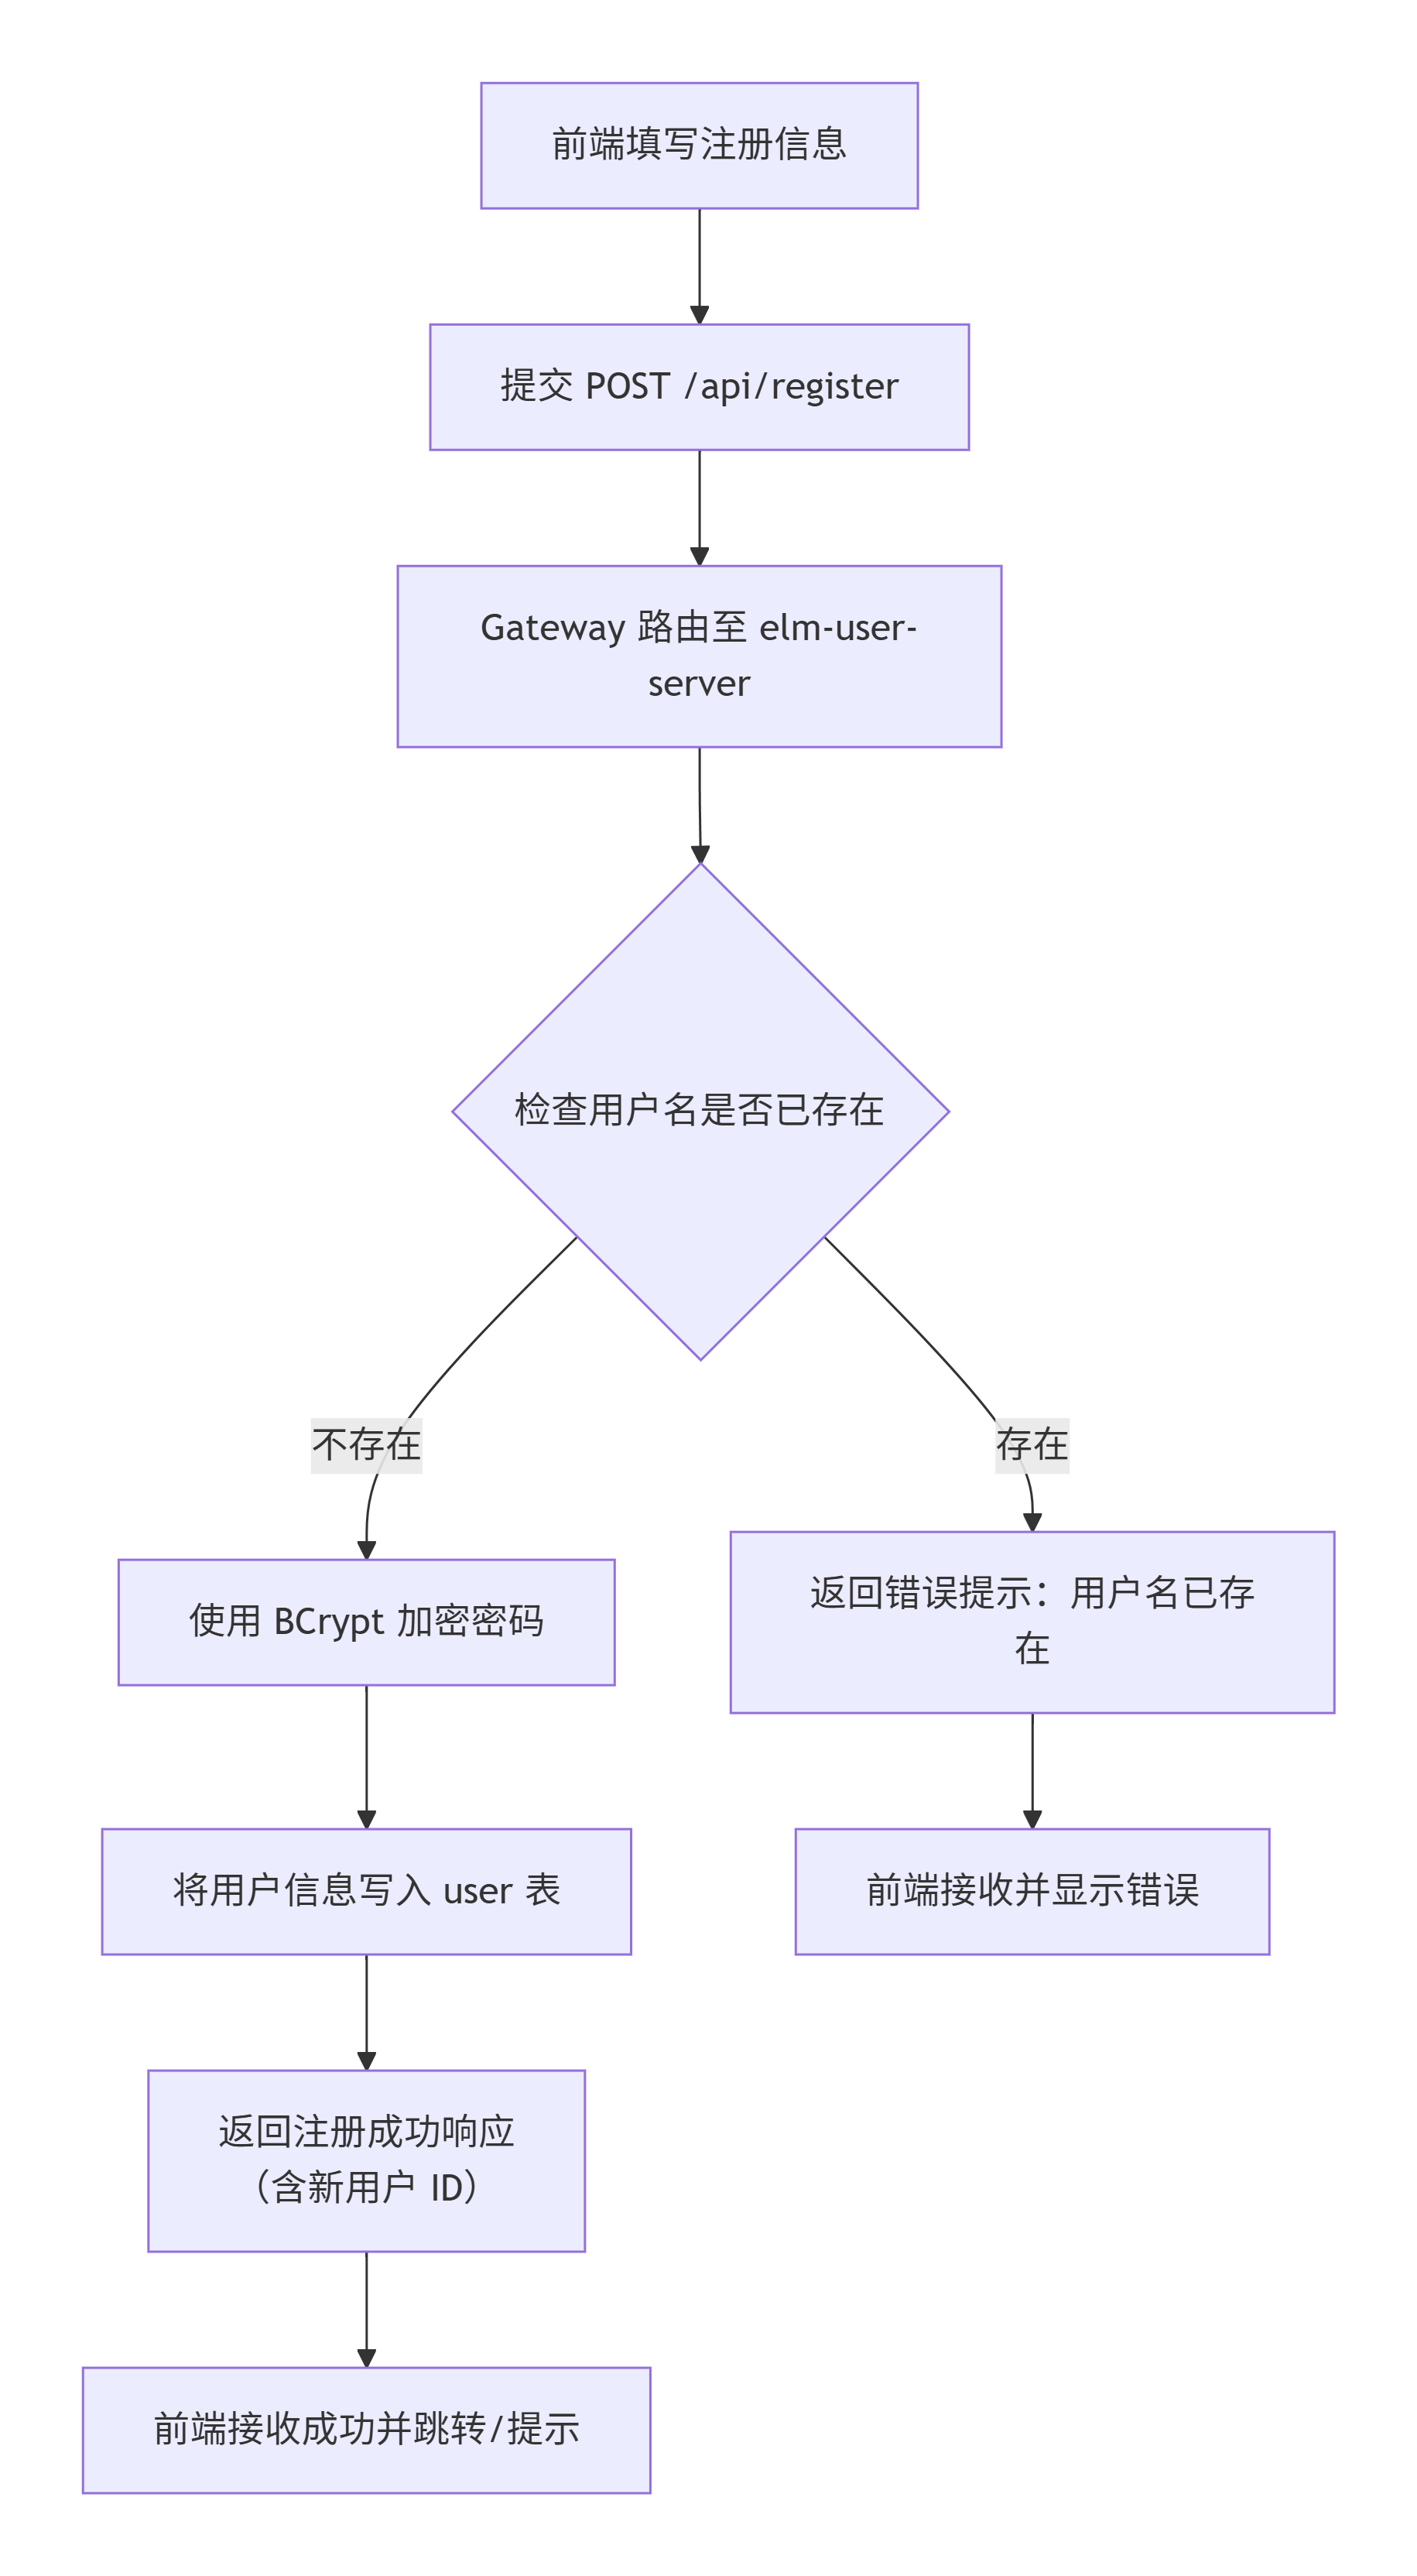
\includegraphics[width=0.75\textwidth,height=0.82\textheight,keepaspectratio]{images/flow-user-register.png}
	\caption{用户注册流程图}
	\label{fig:user-register-flow}
\end{figure}

用户注册流程：用户在前端填写用户名、密码等注册信息后提交POST请求至\verb|/api/register|，请求经Gateway路由至elm-user-server。服务首先检查用户名是否已存在，若不存在则使用BCrypt算法对密码进行哈希加密，将用户信息写入user表，返回注册成功响应（含新用户ID）。若用户名已存在则返回错误提示。

\begin{figure}[H]
	\centering
	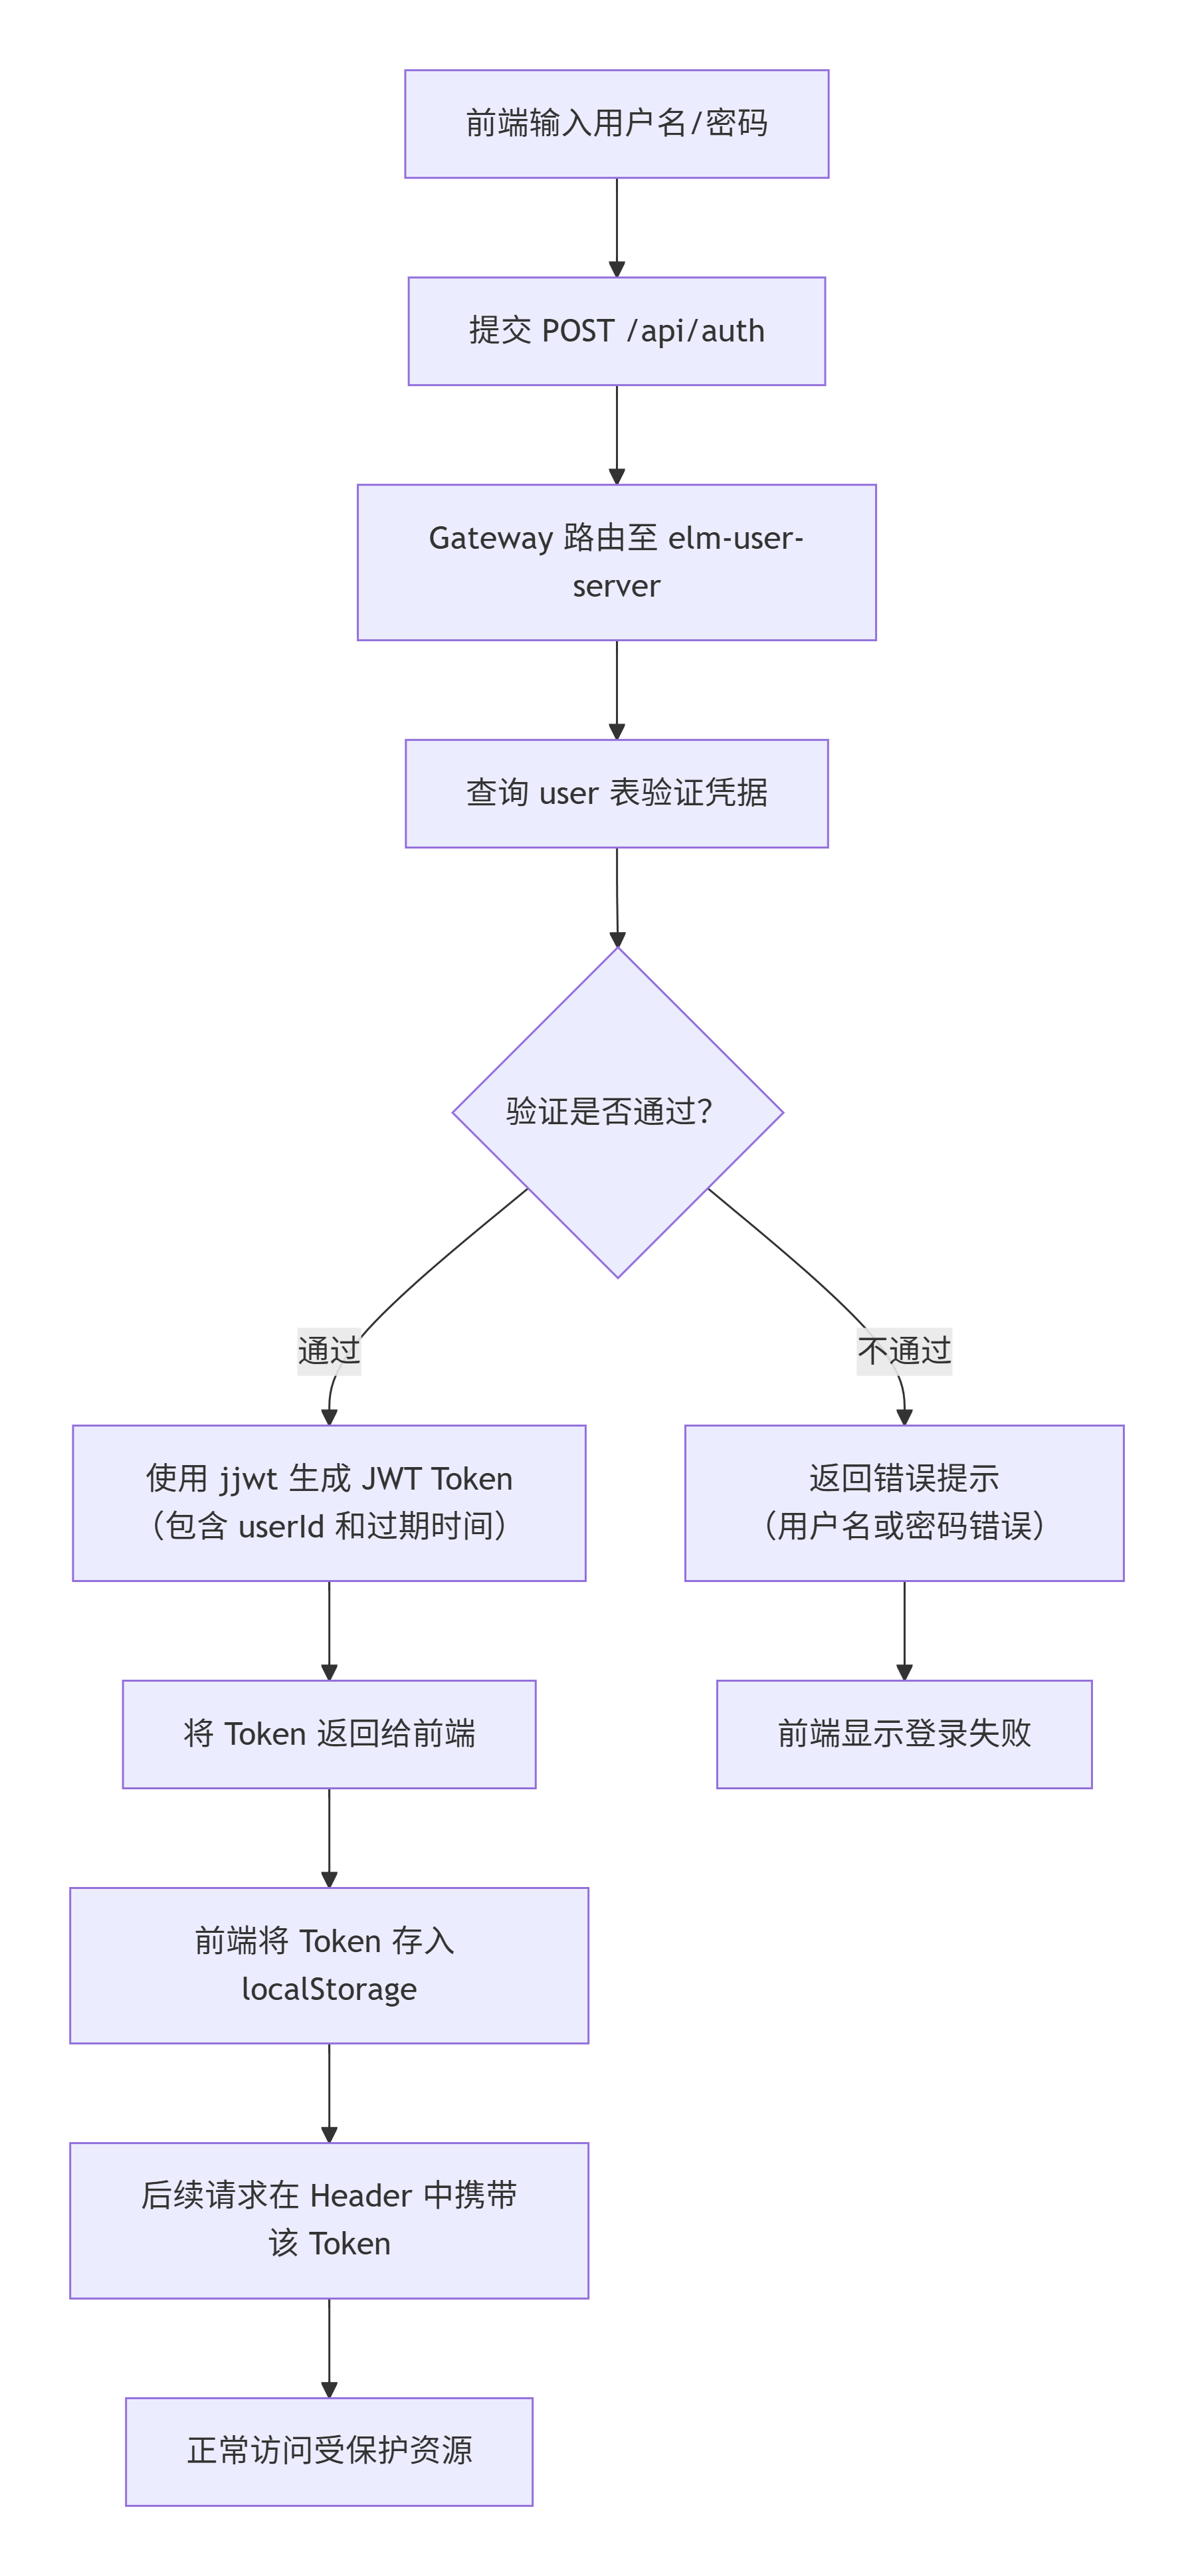
\includegraphics[width=0.75\textwidth,height=0.82\textheight,keepaspectratio]{images/flow-user-login.png}
	\caption{用户登录流程图}
	\label{fig:user-login-flow}
\end{figure}

用户登录流程：用户提交用户名和密码至\verb|/api/auth|，Gateway路由至elm-user-server。服务查询user表验证凭据，验证通过后使用jjwt库生成JWT Token（包含userId和过期时间），将Token返回给前端。前端将Token存入localStorage，后续所有请求均在Header中携带该Token。

\begin{figure}[H]
	\centering
	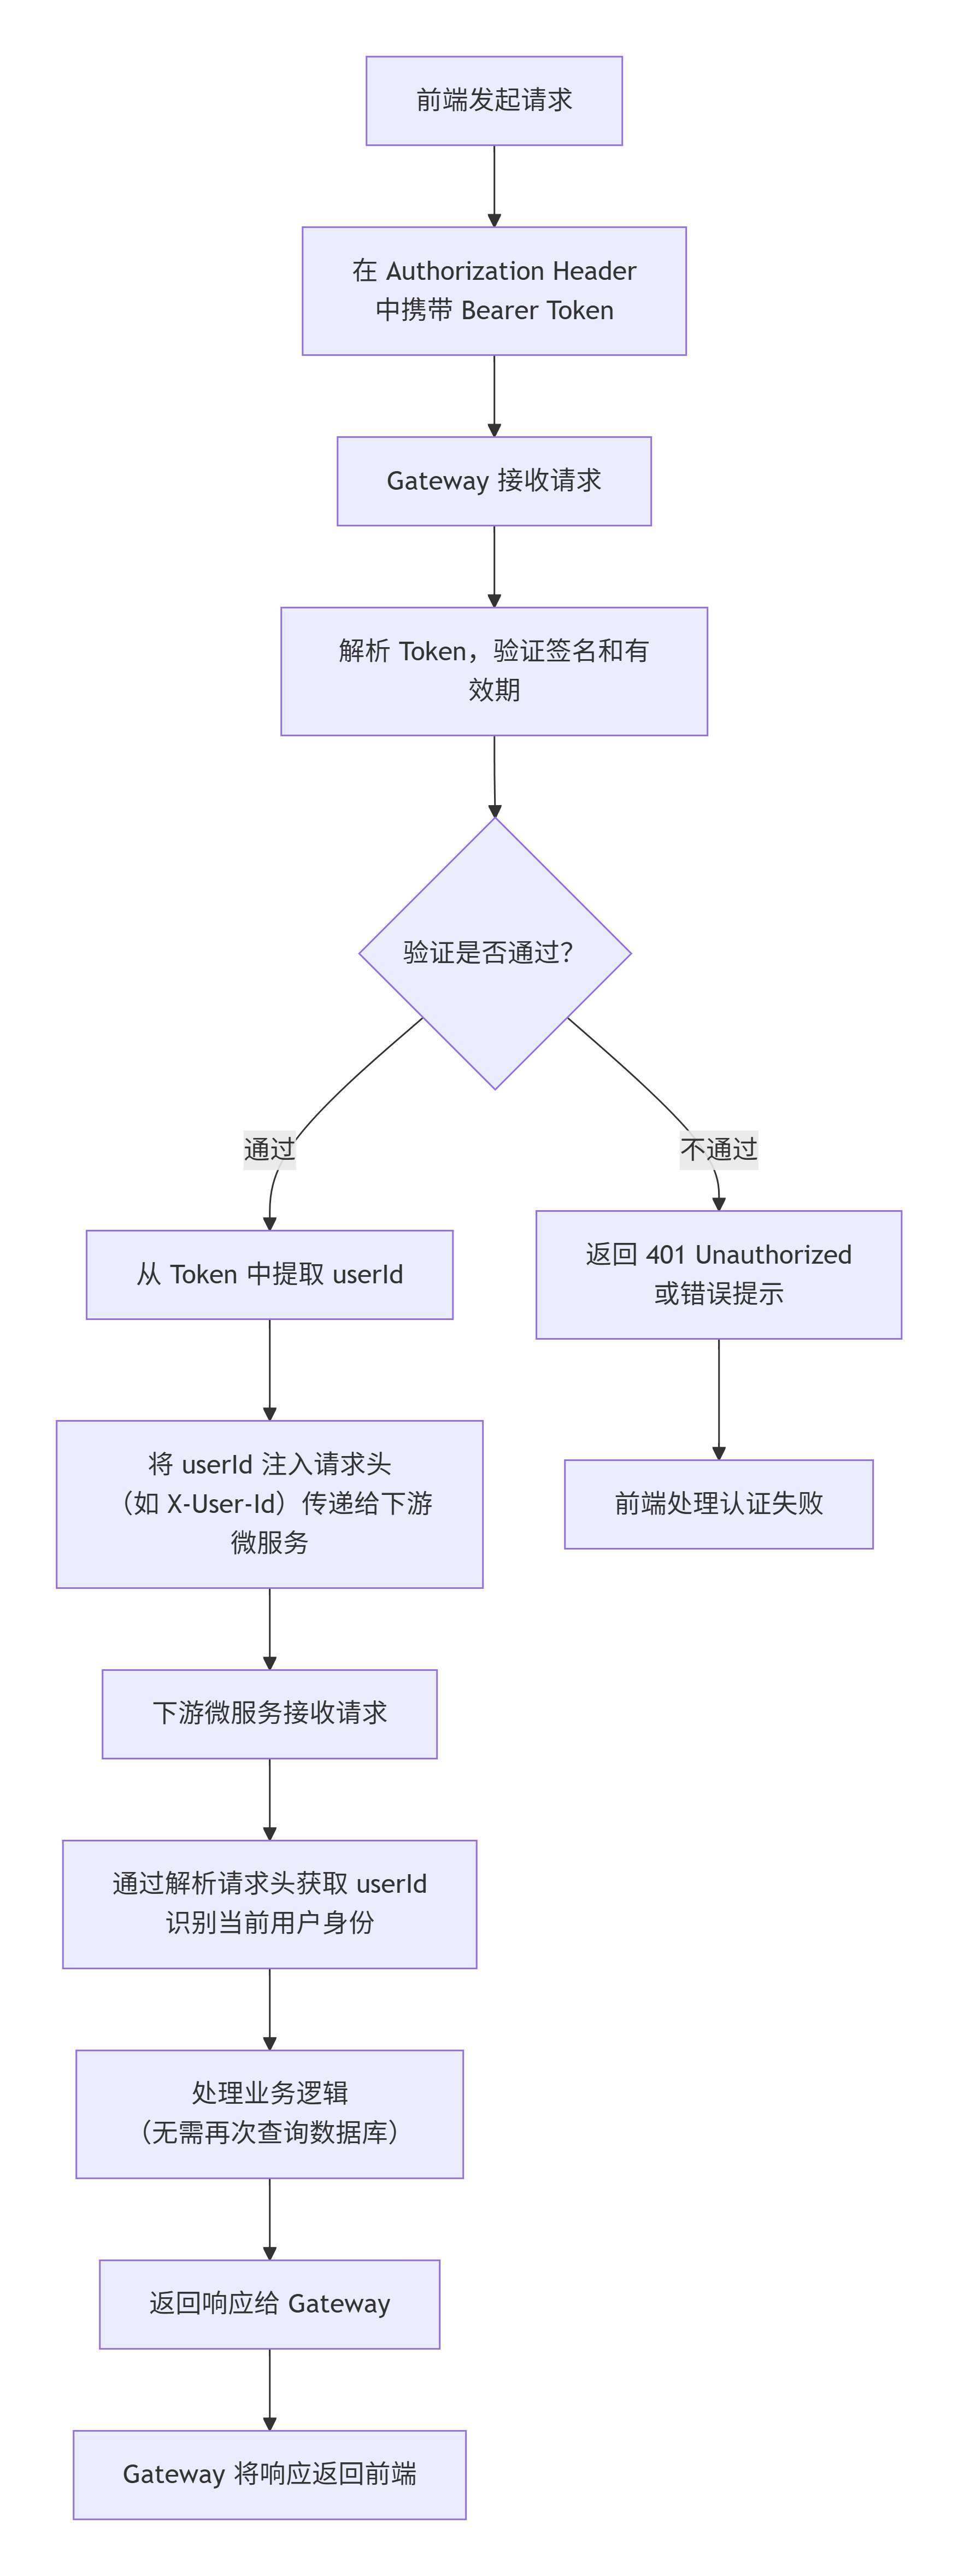
\includegraphics[width=0.75\textwidth,height=0.82\textheight,keepaspectratio]{images/flow-jwt-auth.png}
	\caption{JWT认证流程图}
	\label{fig:jwt-auth-flow}
\end{figure}

JWT认证流程：前端每次请求在Authorization Header中携带Bearer Token，Gateway解析Token验证签名和有效期，从Token中提取userId并注入请求头传递给下游微服务。下游微服务通过解析请求头获取当前用户身份，无需再次查询数据库。

\section{商家微服务 (elm-business-server)}

\begin{longtable}{p{1.5cm}p{2.5cm}p{4.0cm}p{5.5cm}}
	\caption{商家微服务接口一览}\\
	\hline
	\textbf{方法} & \textbf{路径} & \textbf{功能} & \textbf{核心逻辑} \\
	\hline
	\endfirsthead
	GET & /businesses & 获取所有商家 & 列表查询 \\
	GET & /businesses/\{id\} & 按ID获取商家 & 获取商家详情 \\
	GET & /businesses/user/\{id\} & 按用户获取商家 & 获取某用户拥有的商家 \\
	POST & /businesses & 创建商家 & 注册新商家 \\
	PUT & /businesses/\{id\} & 更新商家 & 修改商家信息 \\
	GET & /businesses/order-type/\{id\} & 获取订单类型 & 查询商家订单类型 \\
	POST & /orders & 创建订单 & 创建订单含明细 \\
	GET & /orders/user/\{id\} & 按用户查订单 & 用户订单列表 \\
	GET & /orders/business/\{id\} & 按商家查订单 & 商家订单列表 \\
	GET & /orders/\{id\} & 获取订单详情 & 单个订单 \\
	PUT & /orders/\{id\}/pay & 支付订单 & 状态0→1 \\
	PUT & /orders/\{id\}/deliver & 配送订单 & 状态1→2 \\
	PUT & /orders/\{id\}/checkout & 确认收货 & 状态2→4 \\
	\hline
\end{longtable}

\subsection{商家服务操作流程}

\begin{figure}[H]
	\centering
	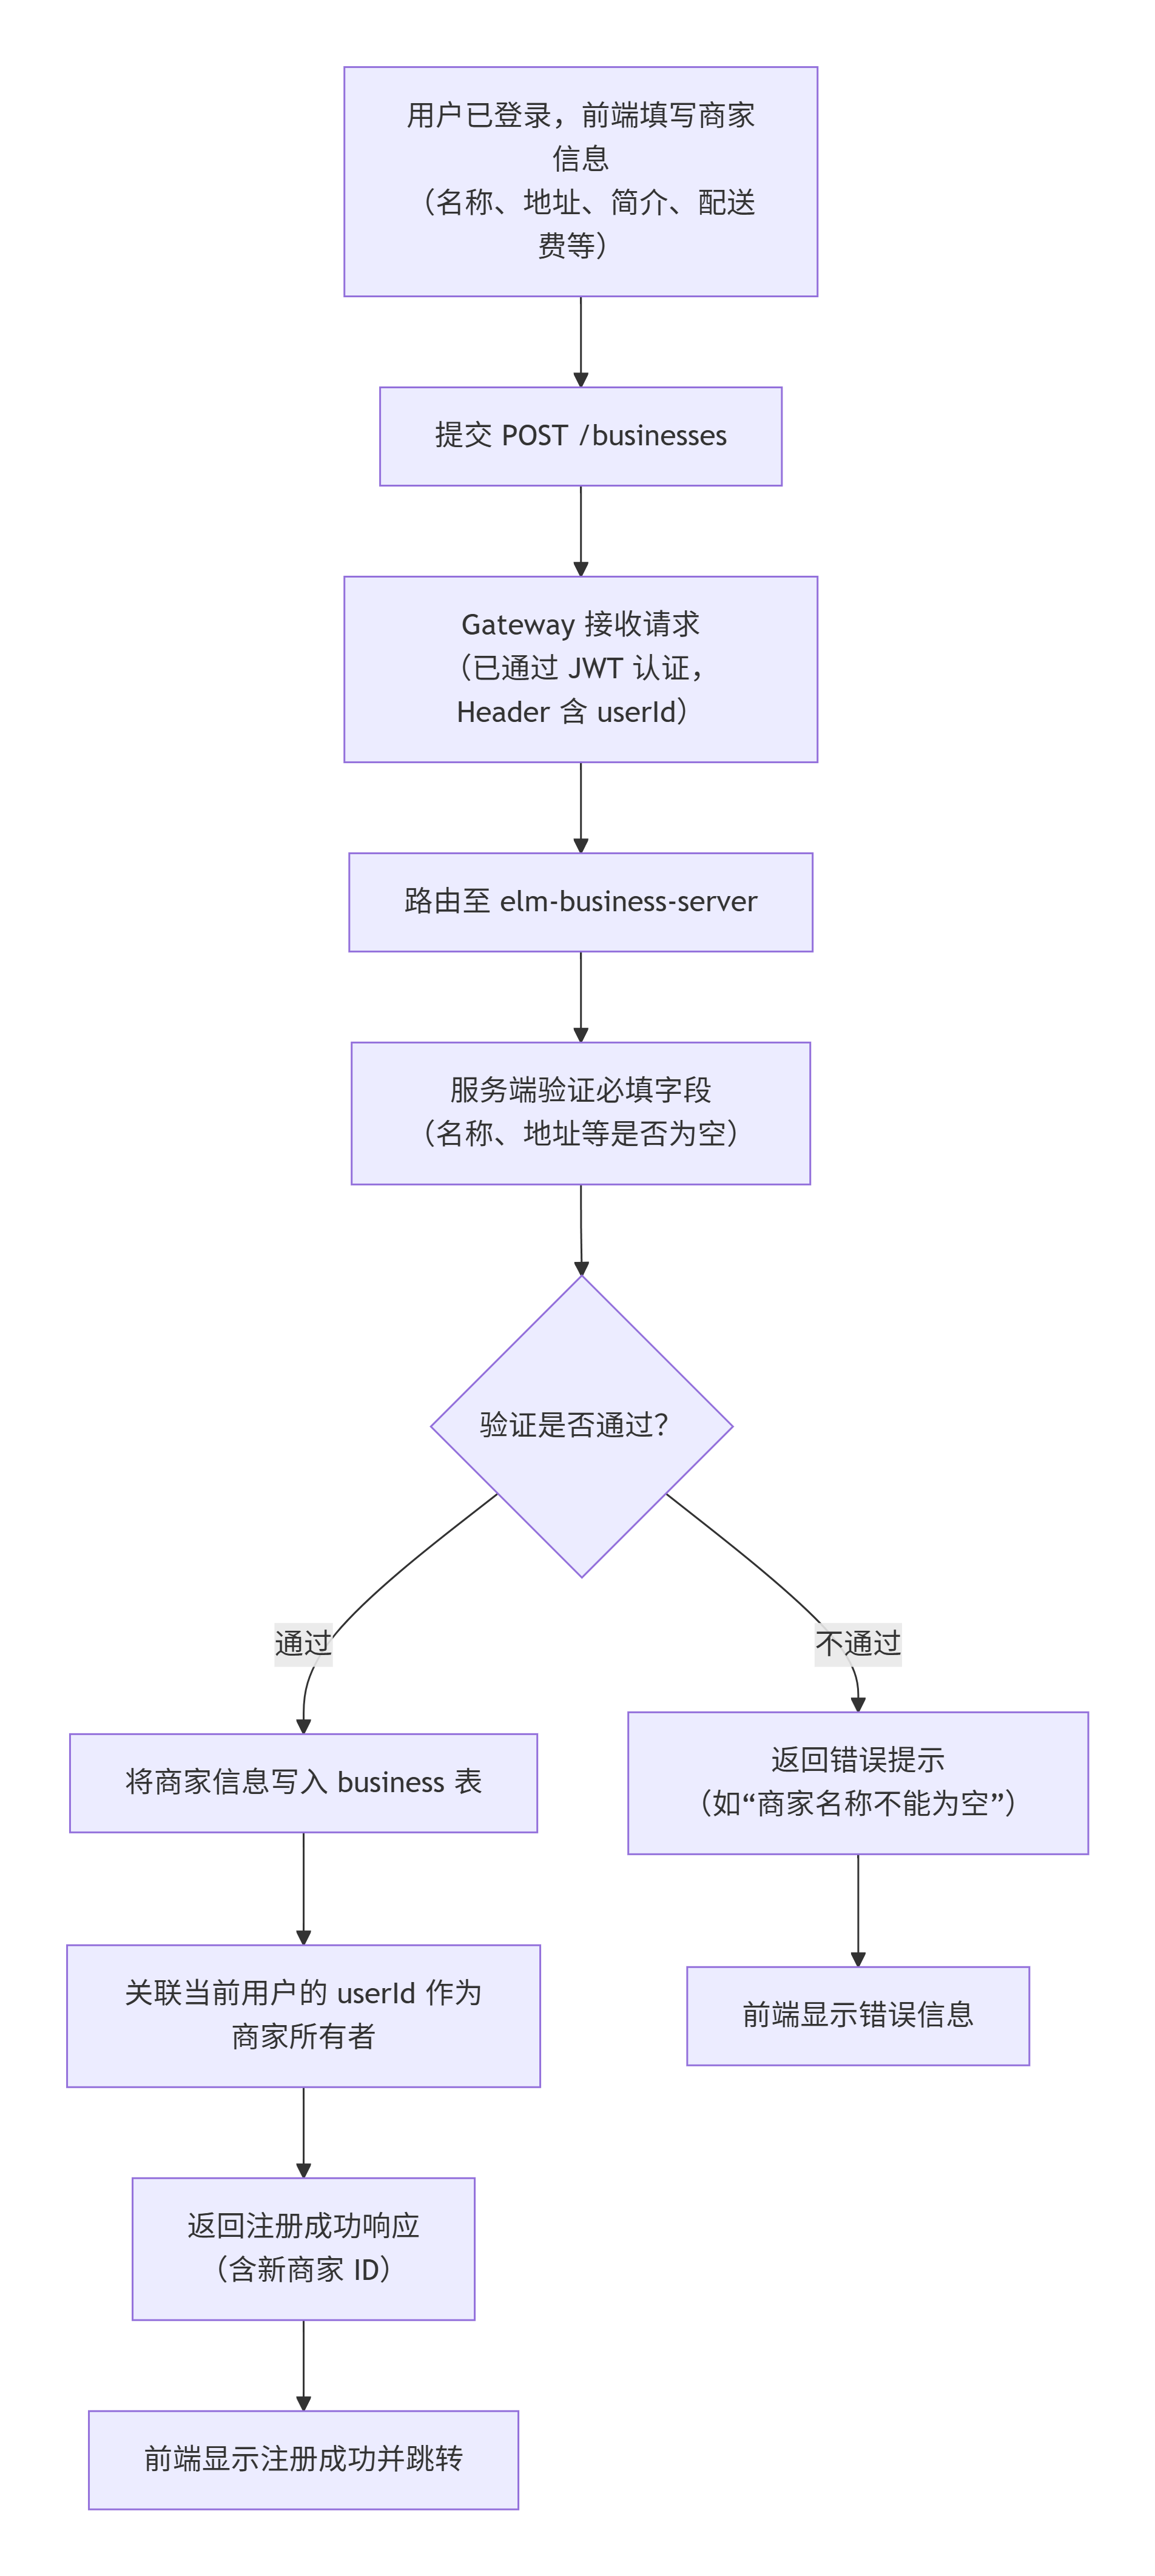
\includegraphics[width=0.75\textwidth,height=0.82\textheight,keepaspectratio]{images/flow-business-register.png}
	\caption{商家注册流程图}
	\label{fig:business-register-flow}
\end{figure}

商家注册流程：用户登录后在前端填写商家信息（名称、地址、简介、配送费等），提交POST请求至\verb|/businesses|。Gateway将请求路由至elm-business-server，服务验证必填字段后将商家信息写入business表，并关联当前用户的userId作为商家所有者。

\begin{figure}[H]
	\centering
	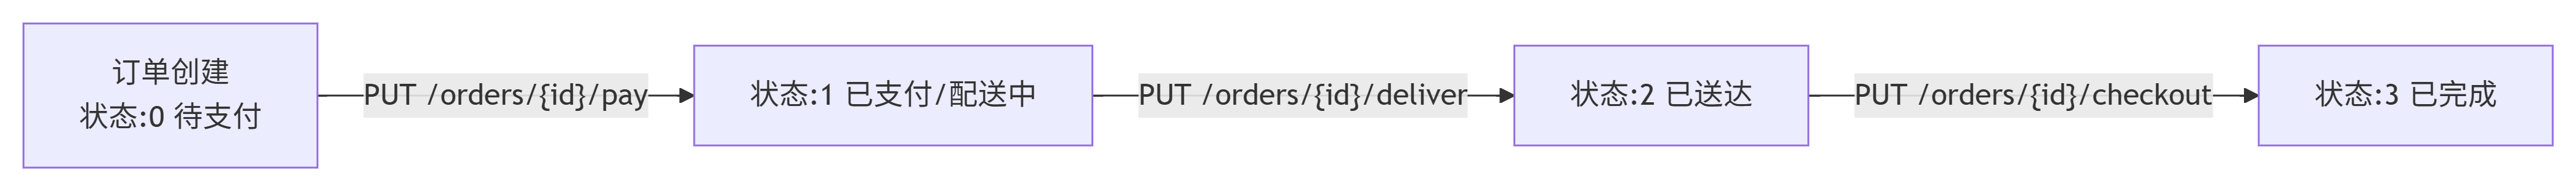
\includegraphics[width=0.75\textwidth,height=0.82\textheight,keepaspectratio]{images/flow-order-state.png}
	\caption{订单状态流转图}
	\label{fig:order-state-flow}
\end{figure}

订单状态流转流程：订单创建后初始状态为0（待支付），商家确认后调用\verb|PUT /orders/{id}/pay|将状态更新为1（已支付/配送中），配送完成后调用\verb|PUT /orders/{id}/deliver|更新为2（已送达），用户确认收货后调用\verb|PUT /orders/{id}/checkout|更新为4（已确认收货）。

\section{食品微服务 (elm-food-server)}

\begin{longtable}{p{1.5cm}p{2.5cm}p{4.0cm}p{5.5cm}}
	\caption{食品微服务接口一览}\\
	\hline
	\textbf{方法} & \textbf{路径} & \textbf{功能} & \textbf{核心逻辑} \\
	\hline
	\endfirsthead
	GET & /foods & 食品列表 & 按businessId筛选，valid=1 \\
	GET & /foods/\{id\} & 按ID查食品 & 获取食品详情 \\
	POST & /foods & 新增食品 & 创建食品，Feign验证商家存在 \\
	PUT & /foods/\{id\} & 更新食品 & 修改食品信息 \\
	DELETE & /foods/\{id\} & 删除食品 & 逻辑删除(valid=0) \\
	\hline
\end{longtable}

\subsection{食品服务操作流程}

\begin{figure}[H]
	\centering
	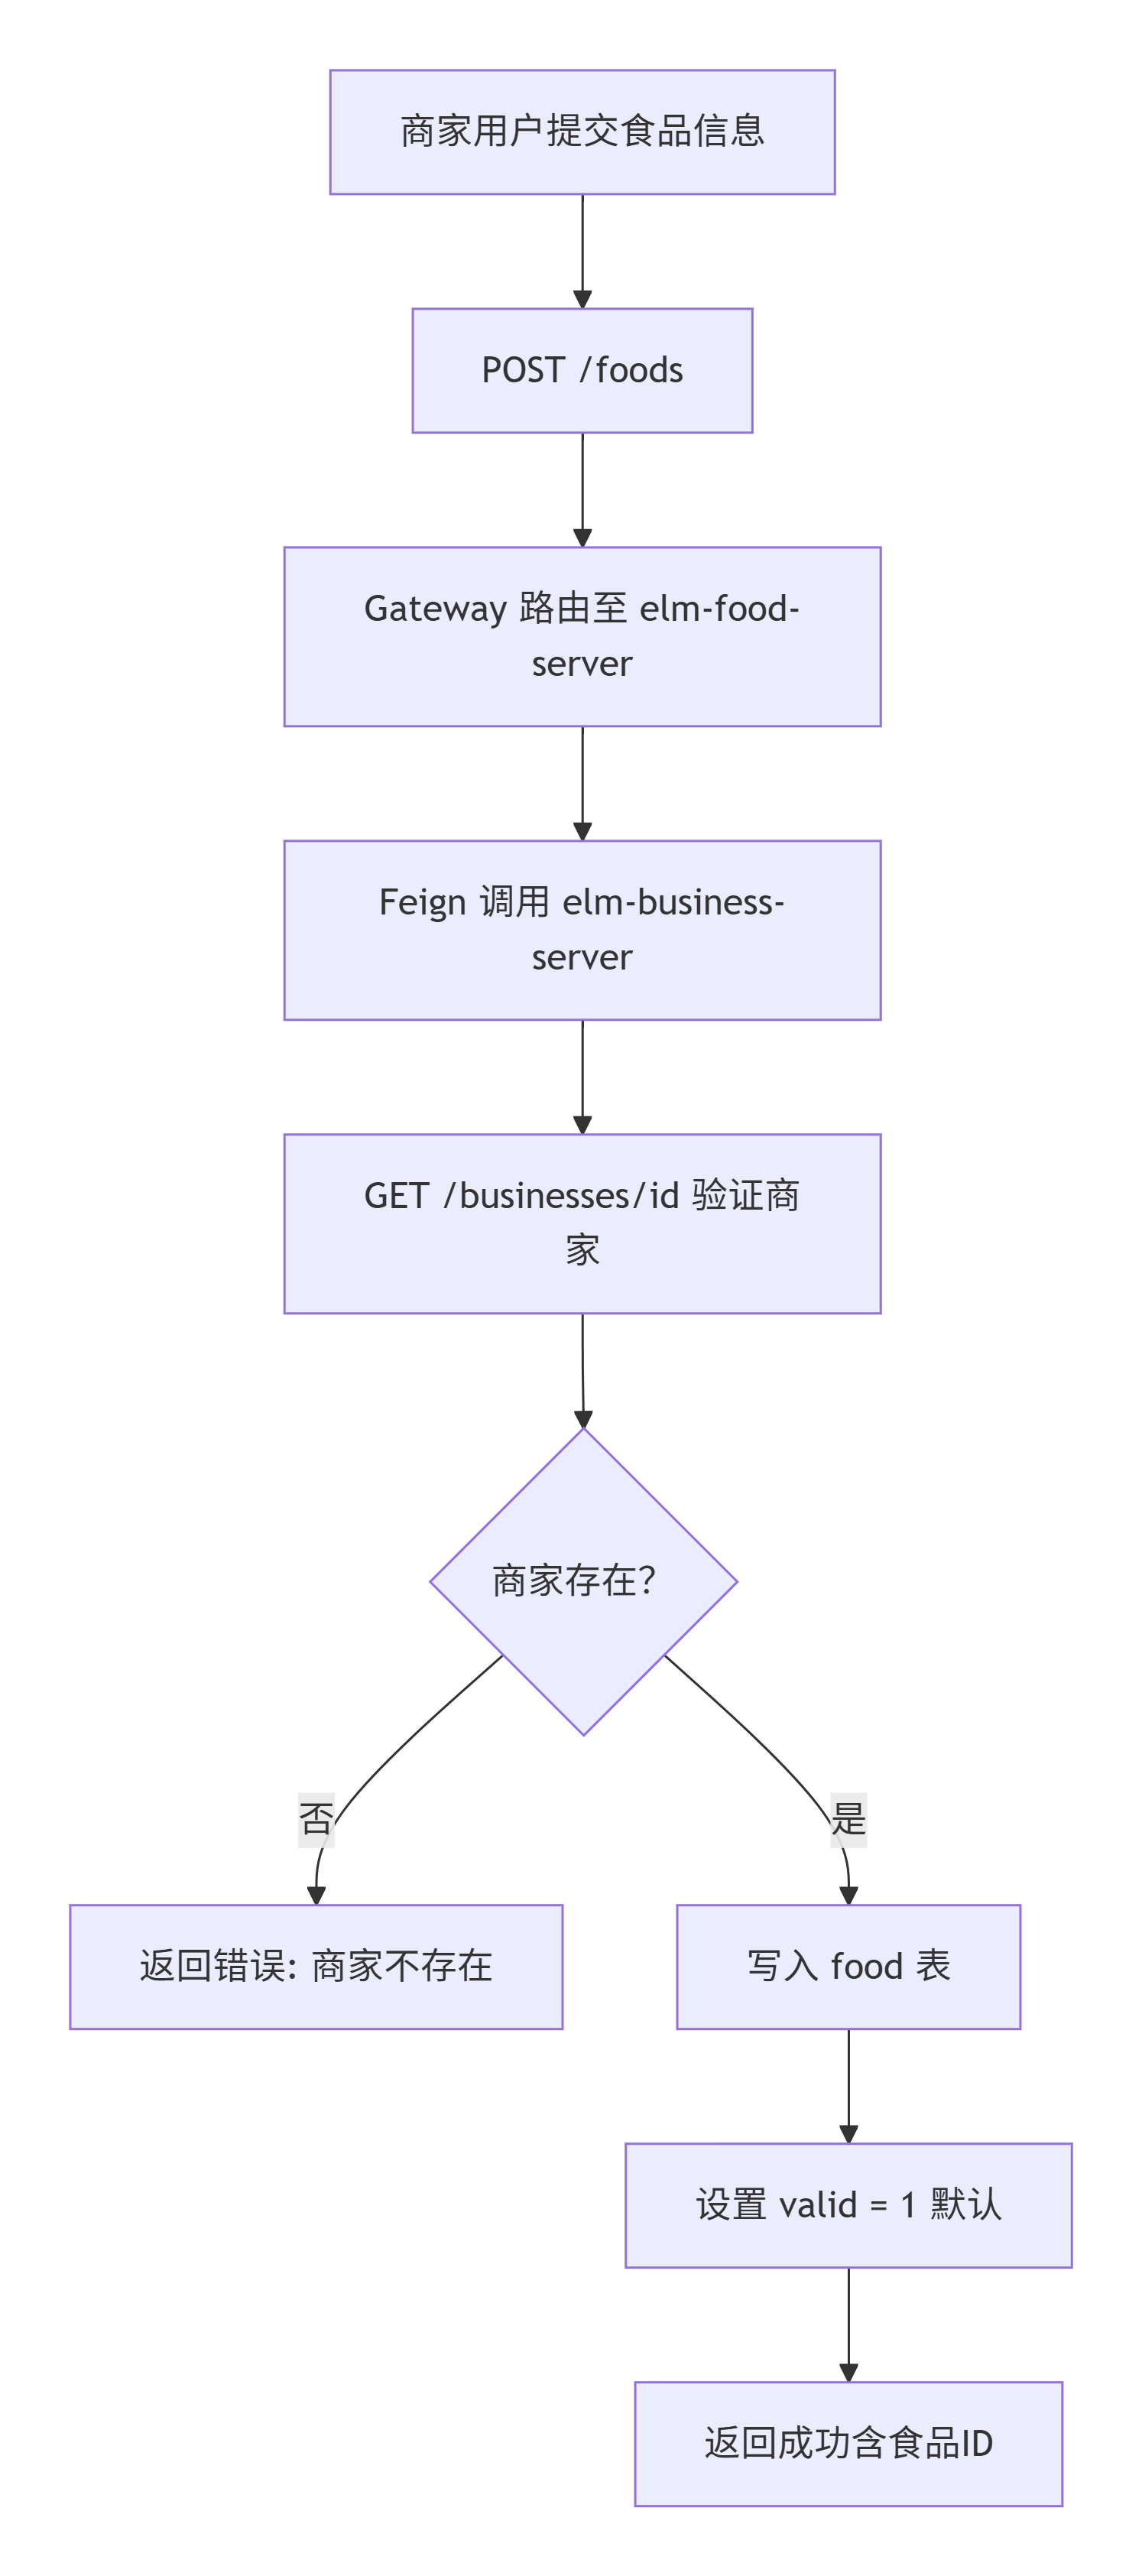
\includegraphics[width=0.75\textwidth,height=0.82\textheight,keepaspectratio]{images/flow-food-manage.png}
	\caption{食品新增流程图}
	\label{fig:food-manage-flow}
\end{figure}

\begin{figure}[H]
	\centering
	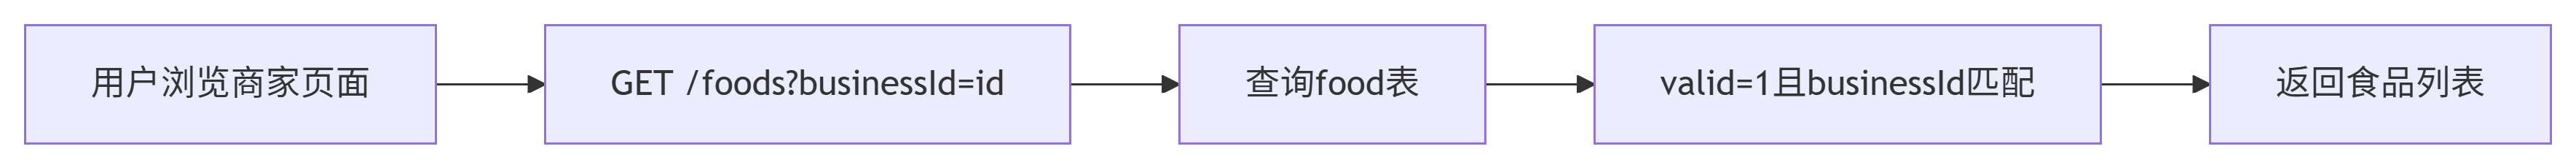
\includegraphics[width=0.75\textwidth,height=0.82\textheight,keepaspectratio]{images/flow-food-query.png}
	\caption{食品查询流程图}
	\label{fig:food-query-flow}
\end{figure}

食品新增流程：商家用户提交食品信息（名称、价格BigDecimal、图片、所属商家ID等）至\verb|POST /foods|。elm-food-server通过Feign客户端调用elm-business-server的\verb|/businesses/{id}|接口验证商家是否存在，验证通过后将食品信息写入food表，valid默认为1。

食品查询流程：用户浏览商家页面时，前端请求\verb|GET /foods?businessId={id}|获取该商家的食品列表。服务查询food表中\verb|valid=1|且\verb|businessId|匹配的记录并返回。

\section{购物车微服务 (elm-cart-server)}

\begin{longtable}{p{1.5cm}p{2.5cm}p{4.0cm}p{5.5cm}}
	\caption{购物车微服务接口一览}\\
	\hline
	\textbf{方法} & \textbf{路径} & \textbf{功能} & \textbf{核心逻辑} \\
	\hline
	\endfirsthead
	GET & /carts/user/\{id\} & 用户购物车 & 用户所有购物车项 \\
	GET & /carts/business/\{id\} & 商家购物车 & 某商家下的购物车 \\
	POST & /carts & 添加商品 & 存在则更新数量，否则新增 \\
	PUT & /carts/\{id\} & 更新数量 & 修改数量 \\
	DELETE & /carts/\{id\} & 删除项目 & 移除购物车项 \\
	\hline
\end{longtable}

\subsection{购物车服务操作流程}

\begin{figure}[H]
	\centering
	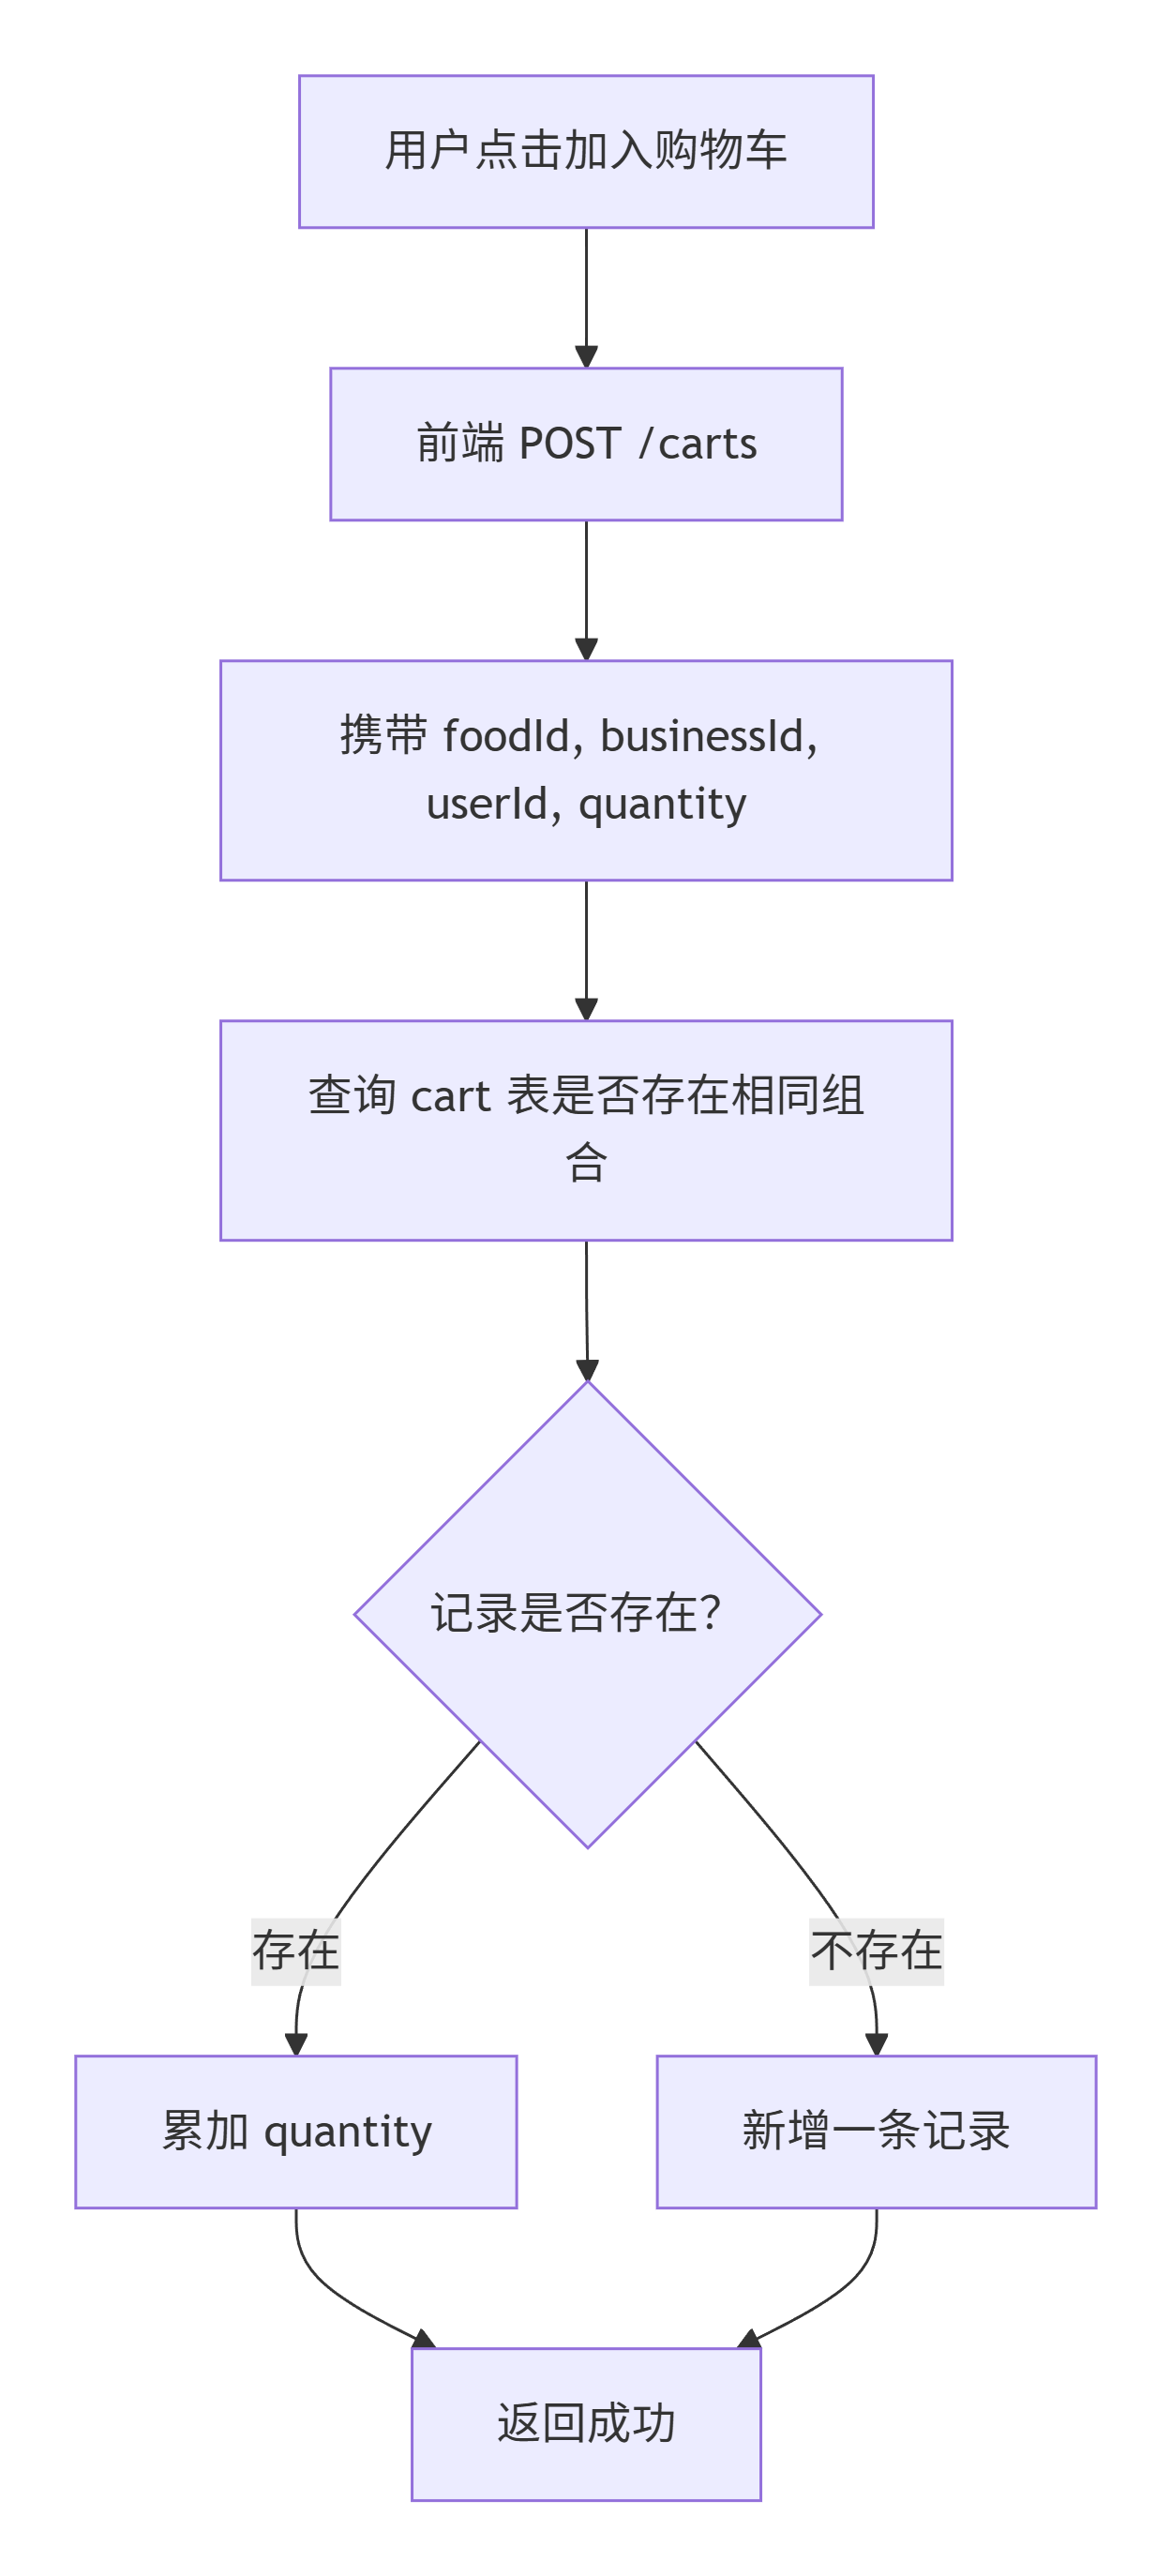
\includegraphics[width=0.75\textwidth,height=0.82\textheight,keepaspectratio]{images/flow-cart-add.png}
	\caption{购物车添加流程图}
	\label{fig:cart-add-flow}
\end{figure}

\begin{figure}[H]
	\centering
	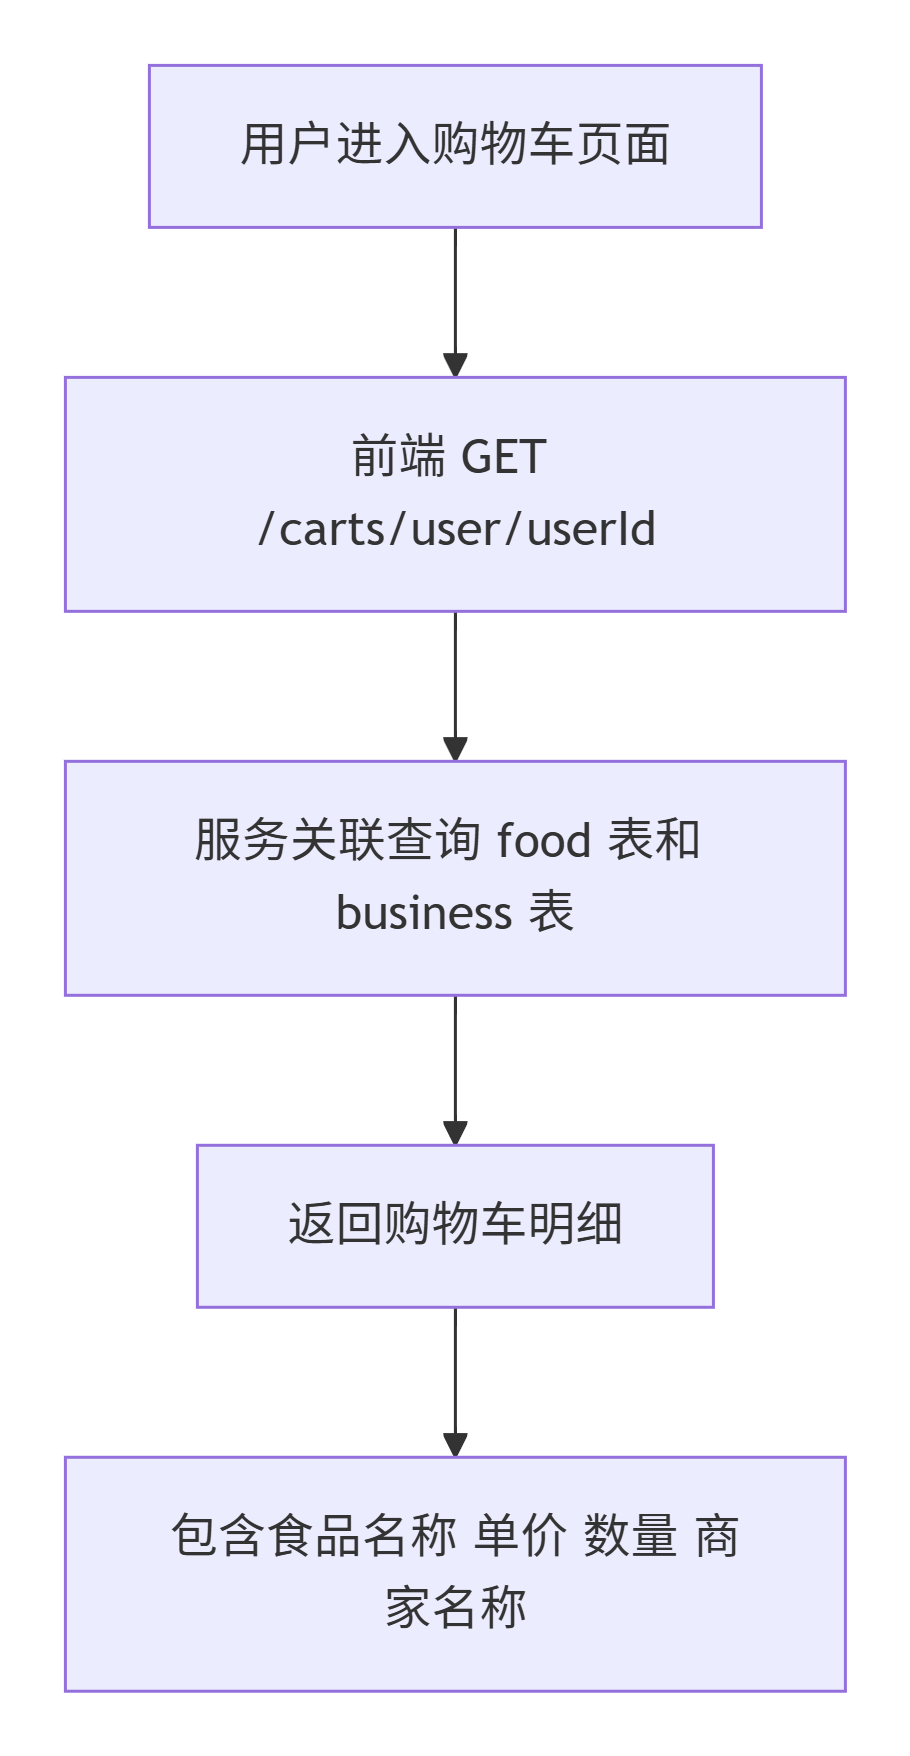
\includegraphics[width=0.75\textwidth,height=0.82\textheight,keepaspectratio]{images/flow-cart-query.png}
	\caption{购物车查询流程图}
	\label{fig:cart-query-flow}
\end{figure}

添加商品流程：用户在食品列表页点击"加入购物车"，前端发送POST请求至\verb|/carts|，携带foodId、businessId、userId和quantity。elm-cart-server查询cart表中是否存在相同的(foodId, businessId, userId)组合——若存在则累加quantity，若不存在则新增一条cart记录。

购物车查询流程：用户进入购物车页面时，前端请求\verb|GET /carts/user/{userId}|获取该用户所有购物车项。服务关联查询food和business表，返回包含食品名称、单价、数量及商家名称的购物车明细。

\section{订单微服务 (elm-order-server)}

\begin{longtable}{p{1.5cm}p{2.8cm}p{4.0cm}p{5.2cm}}
	\caption{订单微服务接口一览}\\
	\hline
	\textbf{方法} & \textbf{路径} & \textbf{功能} & \textbf{核心逻辑} \\
	\hline
	\endfirsthead
	POST & /orders & 创建订单 & 从购物车创建，集成支付和积分 \\
	GET & /orders/user/\{id\} & 用户订单列表 & 用户所有订单 \\
	GET & /orders/business/\{id\} & 商家订单列表 & 商家收到的订单 \\
	GET & /orders/\{id\} & 获取订单详情 & 单个订单含明细 \\
	PUT & /orders/\{id\}/state & 更新订单状态 & 修改订单状态 \\
	POST & /orders/\{id\}/pay/virtual-wallet & 虚拟钱包支付 & 集成钱包转账+积分抵扣，分布式锁保护 \\
	\hline
\end{longtable}

\subsection{订单服务操作流程}

\begin{figure}[H]
	\centering
	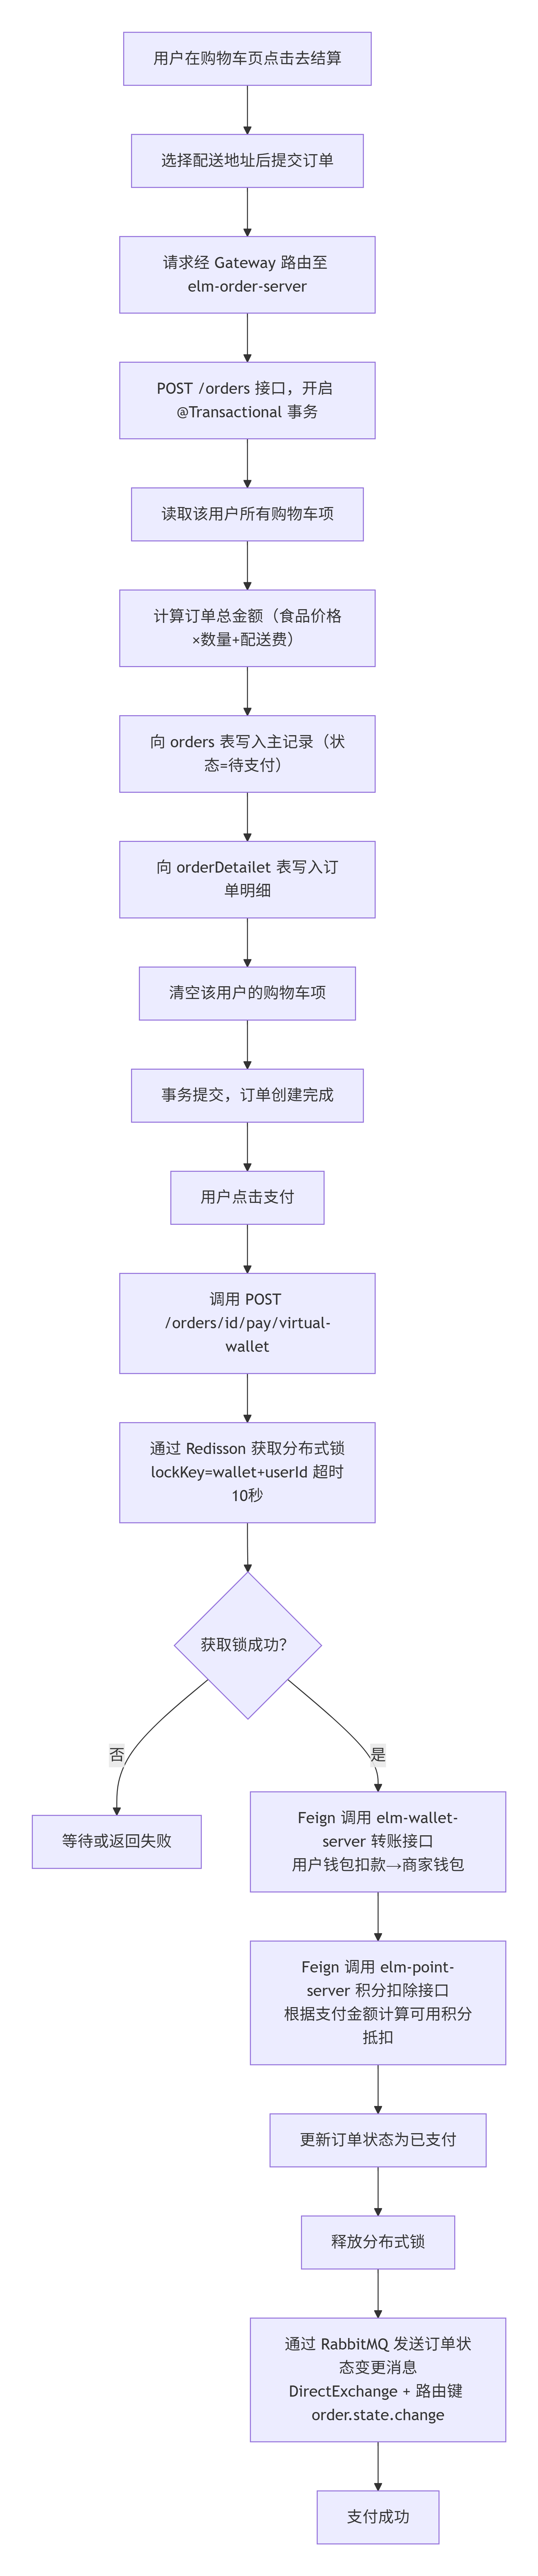
\includegraphics[width=0.75\textwidth,height=0.82\textheight,keepaspectratio]{images/flow-order-create-pay.png}
	\caption{订单创建与支付流程图}
	\label{fig:order-create-pay-flow}
\end{figure}

订单创建与支付流程（核心业务流）：
\begin{enumerate}
	\item 用户在前端购物车页面点击"去结算"，选择配送地址后提交订单
	\item 请求经Gateway路由至elm-order-server的\verb|POST /orders|接口
	\item 服务开启Spring \verb|@Transactional|事务，执行以下步骤：
	\begin{itemize}
		\item 从cart表读取该用户的所有购物车项
		\item 计算订单总金额（食品价格×数量 + 配送费）
		\item 向orders表写入订单主记录（初始状态为待支付）
		\item 向orderDetailet表写入订单明细
		\item 清空该用户的购物车项
	\end{itemize}
	\item 用户点击"支付"，调用\verb|POST /orders/{id}/pay/virtual-wallet|
	\item 服务通过Redisson获取分布式锁（lockKey=wallet+userId，超时10秒）
	\item 在锁保护下执行：
	\begin{itemize}
		\item 通过Feign调用elm-wallet-server的转账接口，从用户钱包扣款至商家钱包
		\item 通过Feign调用elm-point-server的积分扣除接口，根据支付金额计算可用积分抵扣
		\item 更新订单状态为已支付
	\end{itemize}
	\item 释放分布式锁
	\item 通过RabbitMQ发送订单状态变更消息（DirectExchange + 路由键order.state.change）
\end{enumerate}

\section{配送地址微服务 (elm-delivery-server)}

\begin{longtable}{p{1.5cm}p{2.8cm}p{4.0cm}p{5.2cm}}
	\caption{配送地址微服务接口一览}\\
	\hline
	\textbf{方法} & \textbf{路径} & \textbf{功能} & \textbf{核心逻辑} \\
	\hline
	\endfirsthead
	GET & /delivery-addresses/user/\{id\} & 用户地址列表 & 用户所有有效地址 \\
	GET & /delivery-addresses/\{id\} & 按ID查地址 & 单个地址详情 \\
	POST & /delivery-addresses & 新增地址 & 添加配送地址 \\
	PUT & /delivery-addresses/\{id\} & 更新地址 & 修改地址信息 \\
	DELETE & /delivery-addresses/\{id\} & 删除地址 & 逻辑删除(valid=0) \\
	\hline
\end{longtable}

\subsection{配送地址服务操作流程}

\begin{figure}[H]
	\centering
	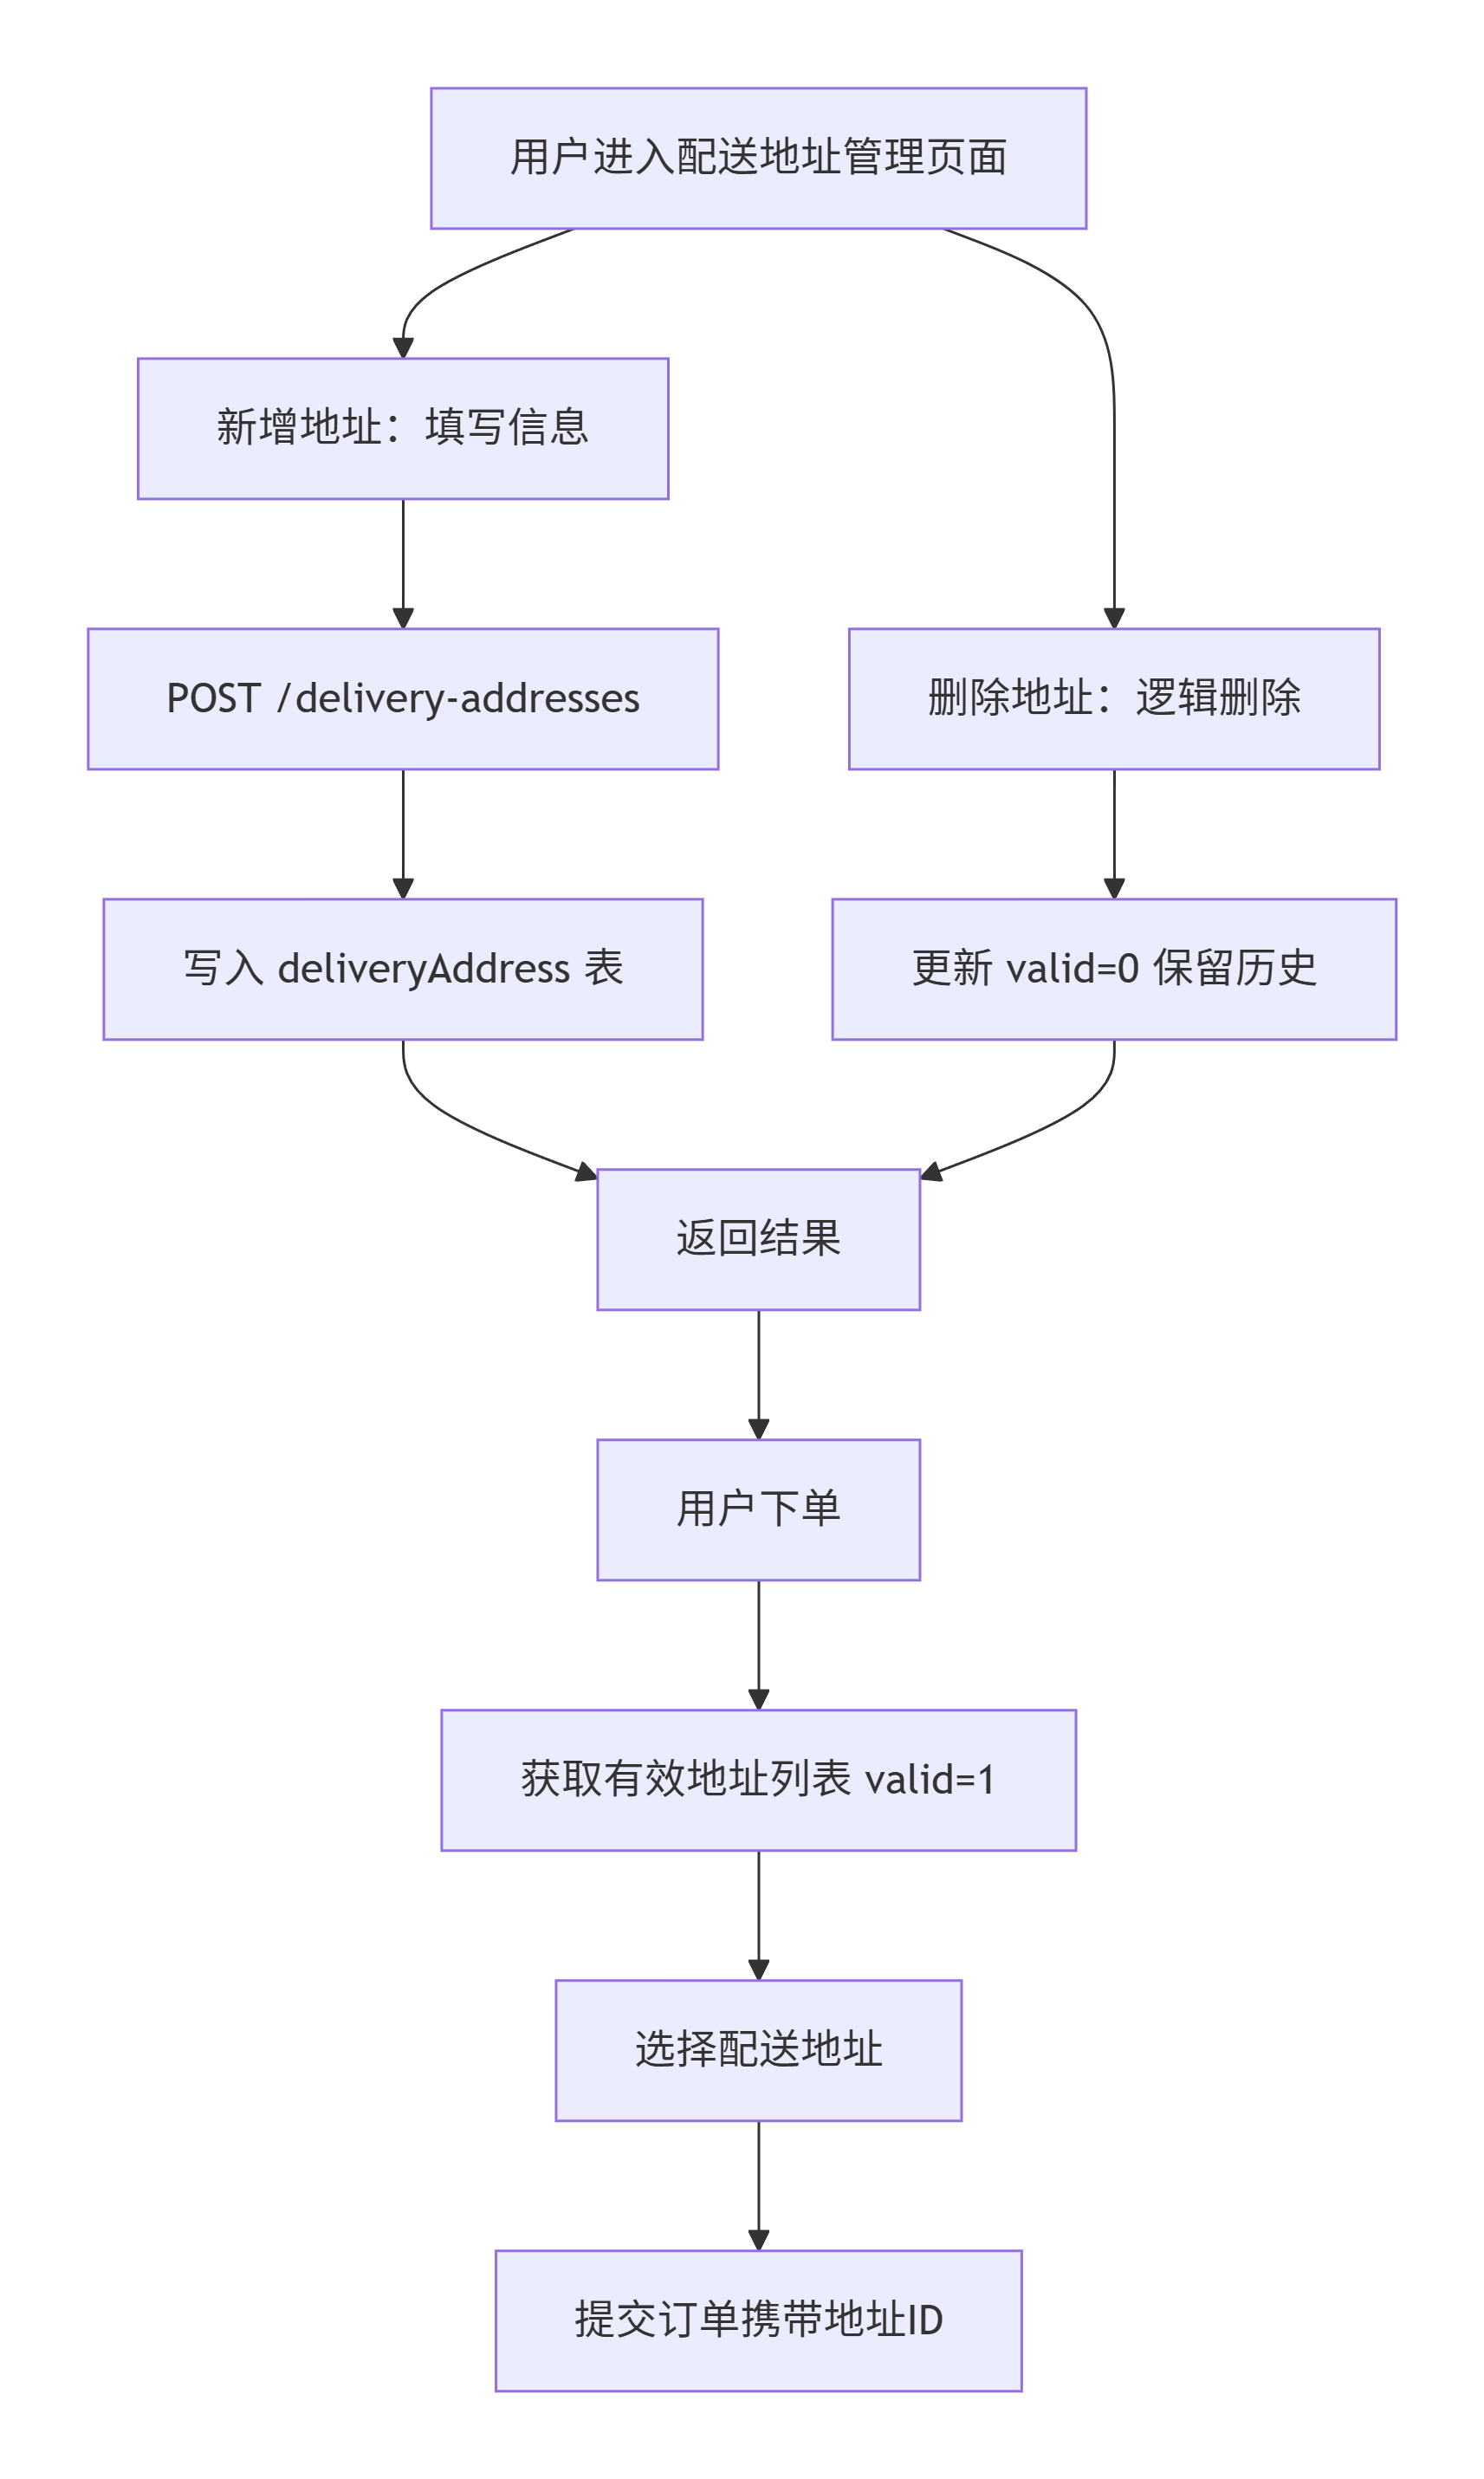
\includegraphics[width=0.75\textwidth,height=0.82\textheight,keepaspectratio]{images/flow-delivery-address.png}
	\caption{配送地址管理流程图}
	\label{fig:delivery-address-flow}
\end{figure}

地址管理流程：用户在下单前可通过配送地址管理页面维护常用地址。新增地址时提交联系人姓名、性别、电话、详细地址至\verb|POST /delivery-addresses|，写入deliveryAddress表。删除地址采用逻辑删除（valid=0），保留历史记录以关联历史订单。下单时用户从有效地址列表中选择一个作为配送地址。

\section{虚拟钱包微服务 (elm-wallet-server)}

\begin{longtable}{p{1.5cm}p{2.8cm}p{4.0cm}p{5.2cm}}
	\caption{虚拟钱包微服务接口一览}\\
	\hline
	\textbf{方法} & \textbf{路径} & \textbf{功能} & \textbf{核心逻辑} \\
	\hline
	\endfirsthead
	GET & /wallet & 获取钱包列表 & 所有钱包 \\
	GET & /wallet/getBalance & 查询余额 & 按userId查询 \\
	POST & /wallet/recharge & 充值 & 增加余额，分布式锁保护 \\
	POST & /wallet/pay & 支付 & 扣减余额 \\
	POST & /wallet/transfer & 转账 & 用户间转账 \\
	POST & /wallet/repayOverdraft & 还款 & 归还透支金额 \\
	POST & /vip/purchase & 购买VIP & 99元/299元VIP卡，设置信用额度2000 \\
	\hline
\end{longtable}

\subsection{钱包服务操作流程}

\begin{figure}[H]
	\centering
	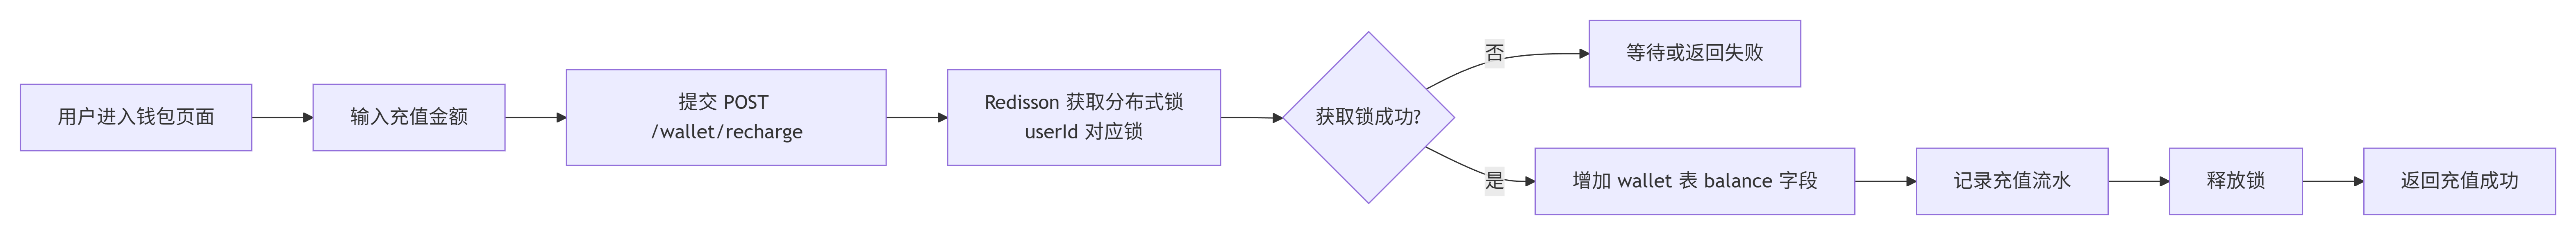
\includegraphics[width=0.75\textwidth,height=0.82\textheight,keepaspectratio]{images/flow-wallet-recharge.png}
	\caption{钱包充值流程图}
	\label{fig:wallet-recharge-flow}
\end{figure}

钱包充值流程：用户进入钱包页面，输入充值金额，提交\verb|POST /wallet/recharge|。服务通过Redisson获取userId对应的分布式锁，在锁保护下增加wallet表中的balance字段，记录充值流水。

\begin{figure}[H]
	\centering
	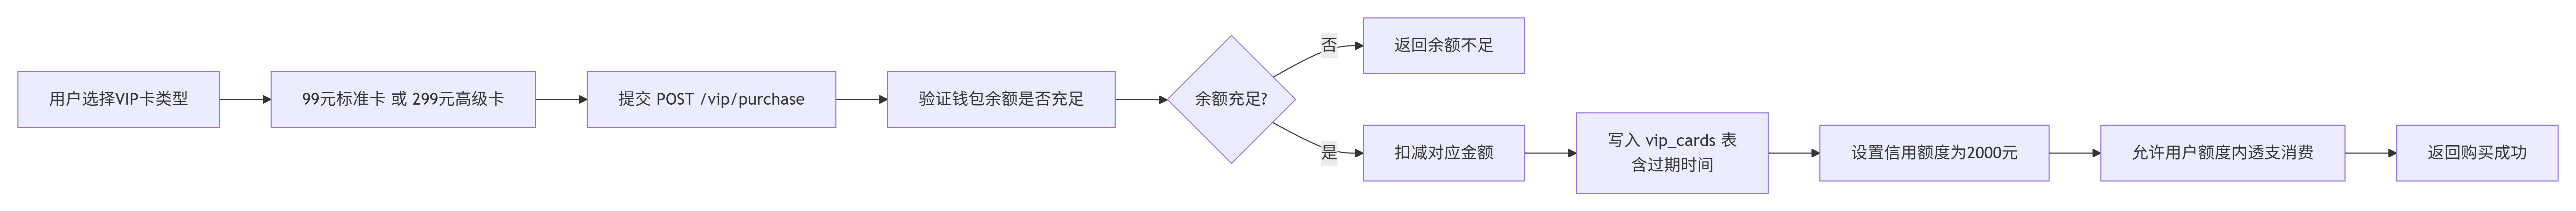
\includegraphics[width=0.75\textwidth,height=0.82\textheight,keepaspectratio]{images/flow-vip-purchase.png}
	\caption{VIP购买流程图}
	\label{fig:vip-purchase-flow}
\end{figure}

VIP购买流程：用户选择VIP卡类型（99元标准卡或299元高级卡），调用\verb|POST /vip/purchase|。服务验证钱包余额充足后扣减对应金额，在vip\_cards表中写入购买记录（含过期时间），同时将信用额度设置为2000元，允许用户在一定额度内透支消费。

\section{积分微服务 (elm-point-server)}

\begin{longtable}{p{1.5cm}p{2.8cm}p{4.0cm}p{5.2cm}}
	\caption{积分微服务接口一览}\\
	\hline
	\textbf{方法} & \textbf{路径} & \textbf{功能} & \textbf{核心逻辑} \\
	\hline
	\endfirsthead
	GET & /integral/available & 查询可用积分 & 用户可用积分余额 \\
	GET & /integral/details & 积分明细 & 积分收支明细 \\
	GET & /integral/statistics & 积分统计 & 总计/可用/已用/过期 \\
	POST & /integral/add & 增加积分 & 管理员发放/活动奖励 \\
	POST & /integral/consume & 消费积分 & 积分消费 \\
	POST & /integral/signIn & 签到 & 每日签到奖励，连续天数越多奖励越多 \\
	POST & /integral/comment & 发表评论 & 评论获积分 \\
	POST & /integral/exchange & 积分兑换 & 积分兑换商品 \\
	GET & /points/balance & 积分余额 & 基础积分余额（Feign用） \\
	POST & /points/earn & 积分赚取 & 基础积分增加（Feign用） \\
	POST & /points/deduct & 积分扣除 & 基础积分扣减（Feign用） \\
	POST/GET & /promotion-day/** & 红包配置 & 红包雨活动管理 \\
	\hline
\end{longtable}

\subsection{积分服务操作流程}

\begin{figure}[H]
	\centering
	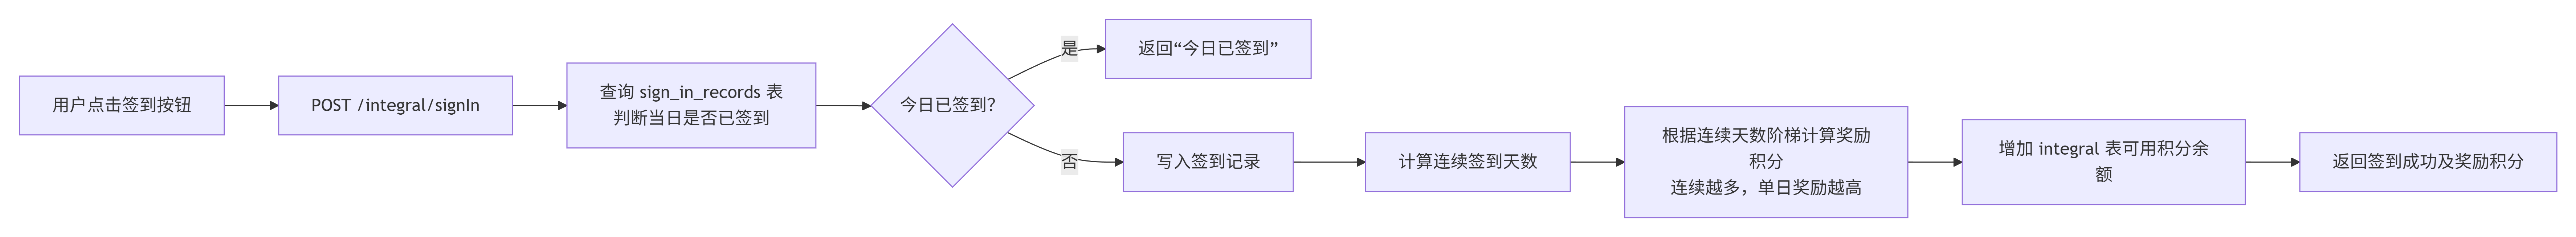
\includegraphics[width=0.75\textwidth,height=0.82\textheight,keepaspectratio]{images/flow-signin.png}
	\caption{每日签到流程图}
	\label{fig:signin-flow}
\end{figure}

每日签到流程：用户每日在前端点击签到按钮，调用\verb|POST /integral/signIn|。服务查询sign\_in\_records表判断当日是否已签到。若未签到则写入签到记录，计算连续签到天数，根据连续天数阶梯计算奖励积分（连续天数越多，单日奖励越高），增加integral表中可用积分余额。

\begin{figure}[H]
	\centering
	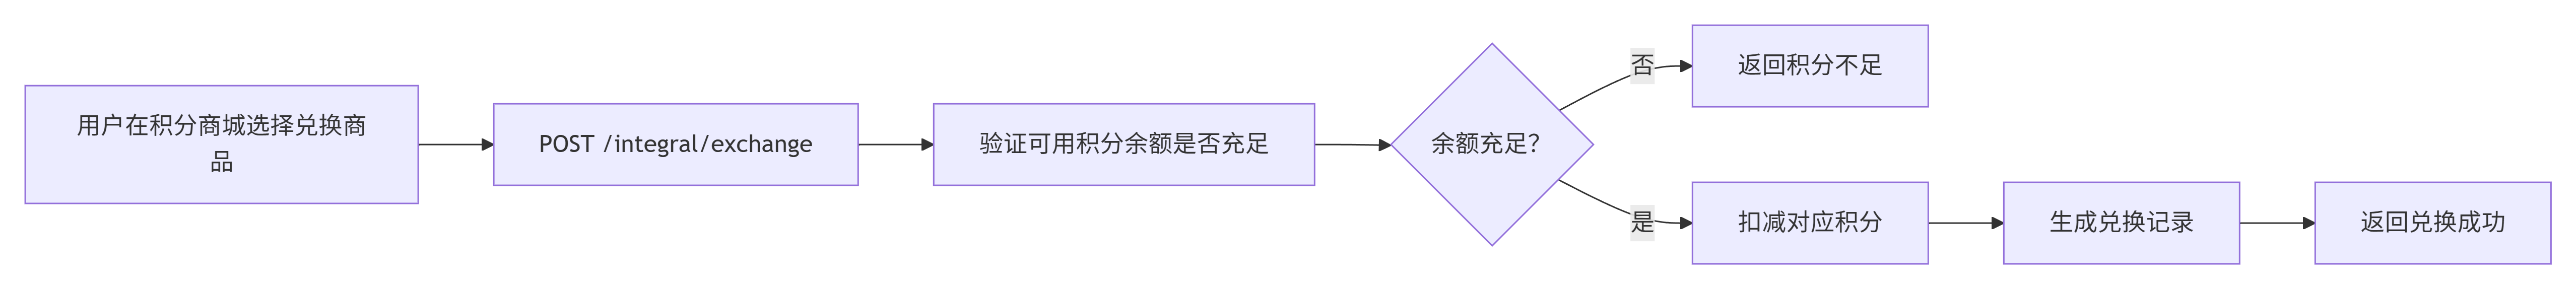
\includegraphics[width=0.75\textwidth,height=0.82\textheight,keepaspectratio]{images/flow-points-exchange.png}
	\caption{积分兑换流程图}
	\label{fig:points-exchange-flow}
\end{figure}

积分兑换流程：用户在积分商城选择兑换商品，调用\verb|POST /integral/exchange|。服务验证可用积分余额是否充足，验证通过后扣减对应积分并生成兑换记录。

\begin{figure}[H]
	\centering
	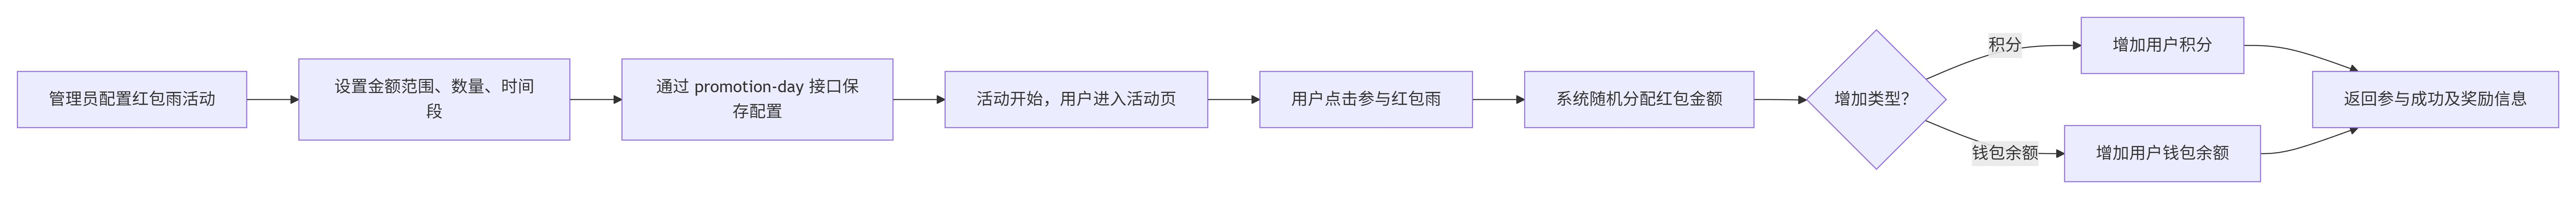
\includegraphics[width=0.75\textwidth,height=0.82\textheight,keepaspectratio]{images/flow-promotion.png}
	\caption{红包雨活动流程图}
	\label{fig:promotion-flow}
\end{figure}

红包雨活动流程：管理员通过promotion-day接口配置红包雨活动（设置红包金额范围、数量、活动时间段）。活动期间用户在前端参与红包雨，系统随机分配红包金额并增加用户积分或钱包余额。

\section{数据库表结构汇总}

系统使用elm2数据库（utf8mb4字符集），核心表包括：

\begin{itemize}
	\item \textbf{user}：userId（主键）、password、userName、userSex、userImg、delTag、userType
	\item \textbf{business}：businessId（自增主键）、businessName、businessAddress、businessExplain、businessImg、orderTypeId、starPrice（DECIMAL）、deliveryPrice（DECIMAL）、remarks、userId
	\item \textbf{food}：foodId（自增主键）、foodName、foodExplain、foodImg、foodPrice（DECIMAL）、businessId、remarks、valid
	\item \textbf{cart}：cartId（自增主键）、foodId、businessId、userId、quantity，唯一约束(foodId,businessId,userId)
	\item \textbf{deliveryAddress}：daId（自增主键）、contactName、contactSex、contactTel、address、userId、valid
	\item \textbf{orders}：orderId（自增主键）、userId、businessId、orderDate、orderTotal（DECIMAL）、daId、orderState
	\item \textbf{orderDetailet}：odId（自增主键）、orderId、foodId、quantity
	\item \textbf{VirtualWallet}：walletId（自增主键）、userId（UNIQUE）、balance（DECIMAL）、creditLimit、usedCreditLimit、lastInterestTime
	\item \textbf{integral}：id（自增主键）、user\_id（VARCHAR(50)）、amount、type、status、channel、expire\_time、business\_id、description、remaining\_amount
	\item \textbf{sign\_in\_records}：id（自增主键）、user\_id（VARCHAR(50)）、sign\_date、consecutive\_days、points\_awarded
	\item \textbf{vip\_cards}：cardId（自增主键）、userId、cardType、price、purchaseTime、expiryTime、status
	\item \textbf{overdraft\_records}：recordId（自增主键）、walletId、overdraftAmount、repaidAmount、dailyInterestRate、status
\end{itemize}
